\chapter{System Architecture}
\label{Chapter4}
\lhead{Chapter 4. \emph{System Architecture}}

Figure~\ref{fig:arch-overview} gives the high-level view. A raw
\texttt{sys\_enter} tracepoint feeds a tail-call dispatcher that routes
each opcode to one of six invariant handlers. A compound gate
\texttt{maybe\_kill(cg, case)} serialises every enforcement request. Tier~2
attributes network traffic to client IPs and severs burned sessions at the
veth. Tier~3 runs the sheaf detector in userspace every detection cycle
and writes verdicts to a JSON log. The three tiers talk to each other only
through shared BPF maps, so Tier~1 never blocks on Tier~3.

\begin{figure}[t]
  \centering
  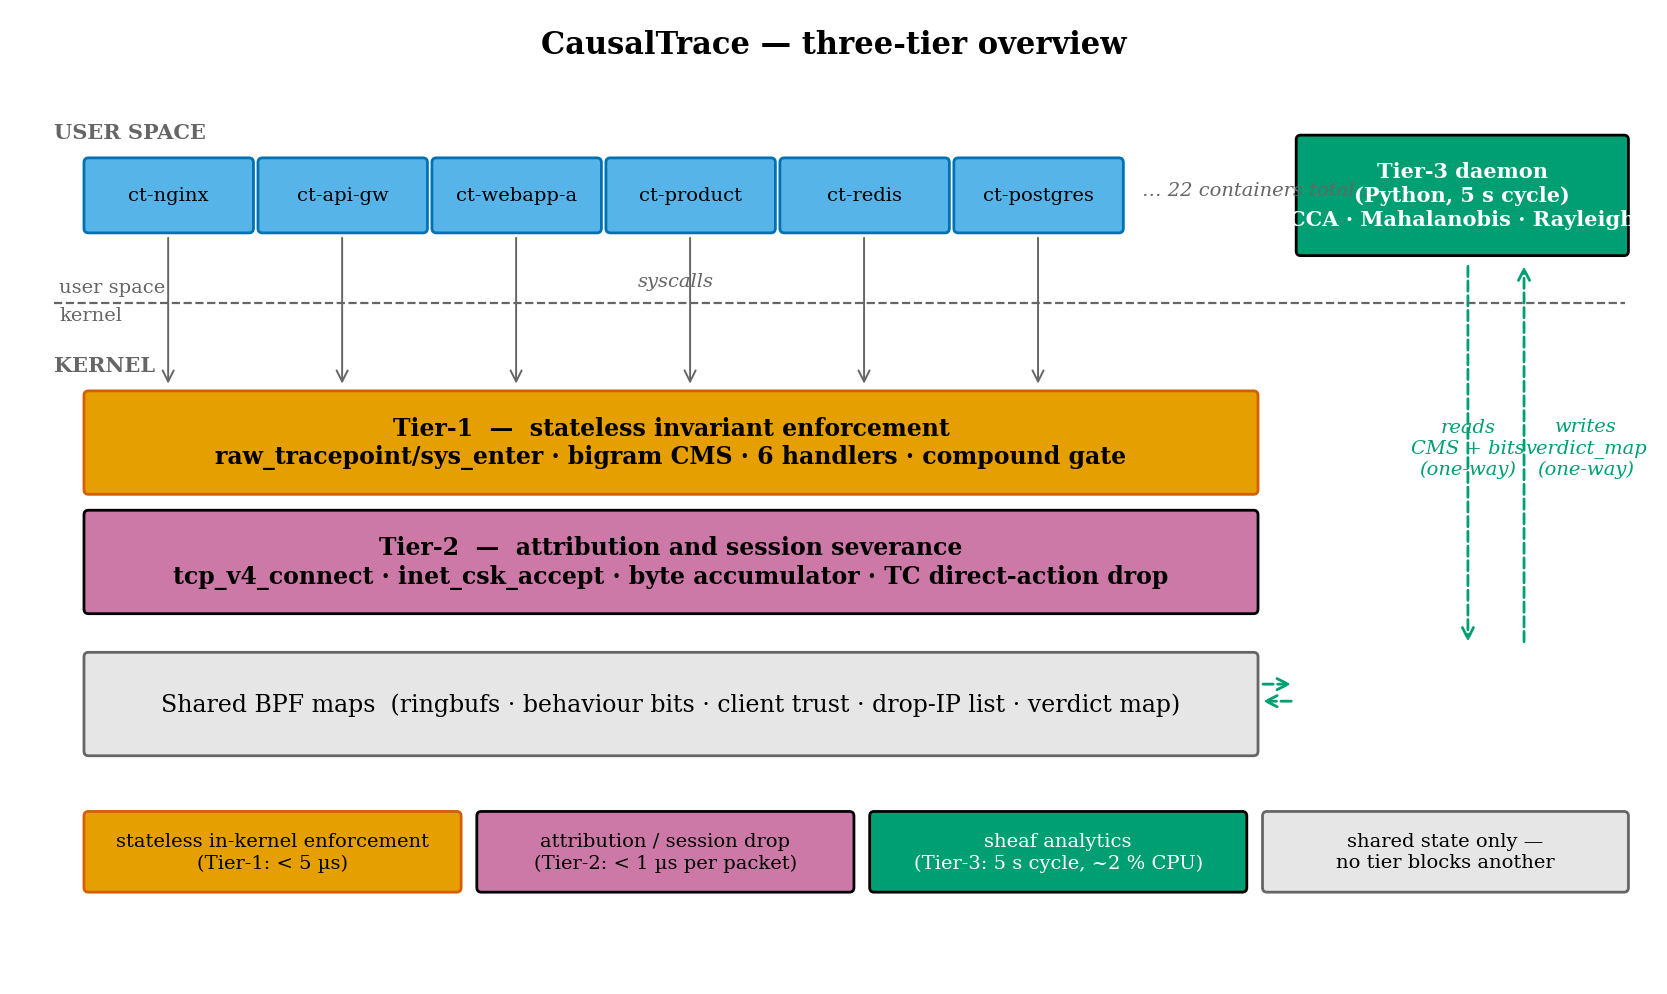
\includegraphics[width=\linewidth]{figures/fig_arch_overview.png}
  \caption[Three-tier overview]{Three-tier overview. Containers sit above the
  user--kernel boundary; Tier~1 (stateless invariant enforcement) and Tier~2
  (attribution + TC drop) live entirely in the kernel; Tier~3 runs in
  userspace and reads state through shared BPF maps only. No tier blocks
  any other tier---if Tier~3 crashes, Tier~1 and Tier~2 keep enforcing.}
  \label{fig:arch-overview}
\end{figure}

Figures~\ref{fig:dataflow-normal} and~\ref{fig:dataflow-attack} trace the
information flow through the three tiers in the two operational regimes we
care about: a benign request that completes normally, and an attack that
fires a strict invariant and burns the attacker's IP. The numbered steps
correspond one-to-one with the implementation paths in Chapter~\ref{Chapter5}.

\begin{figure}[t]
  \centering
  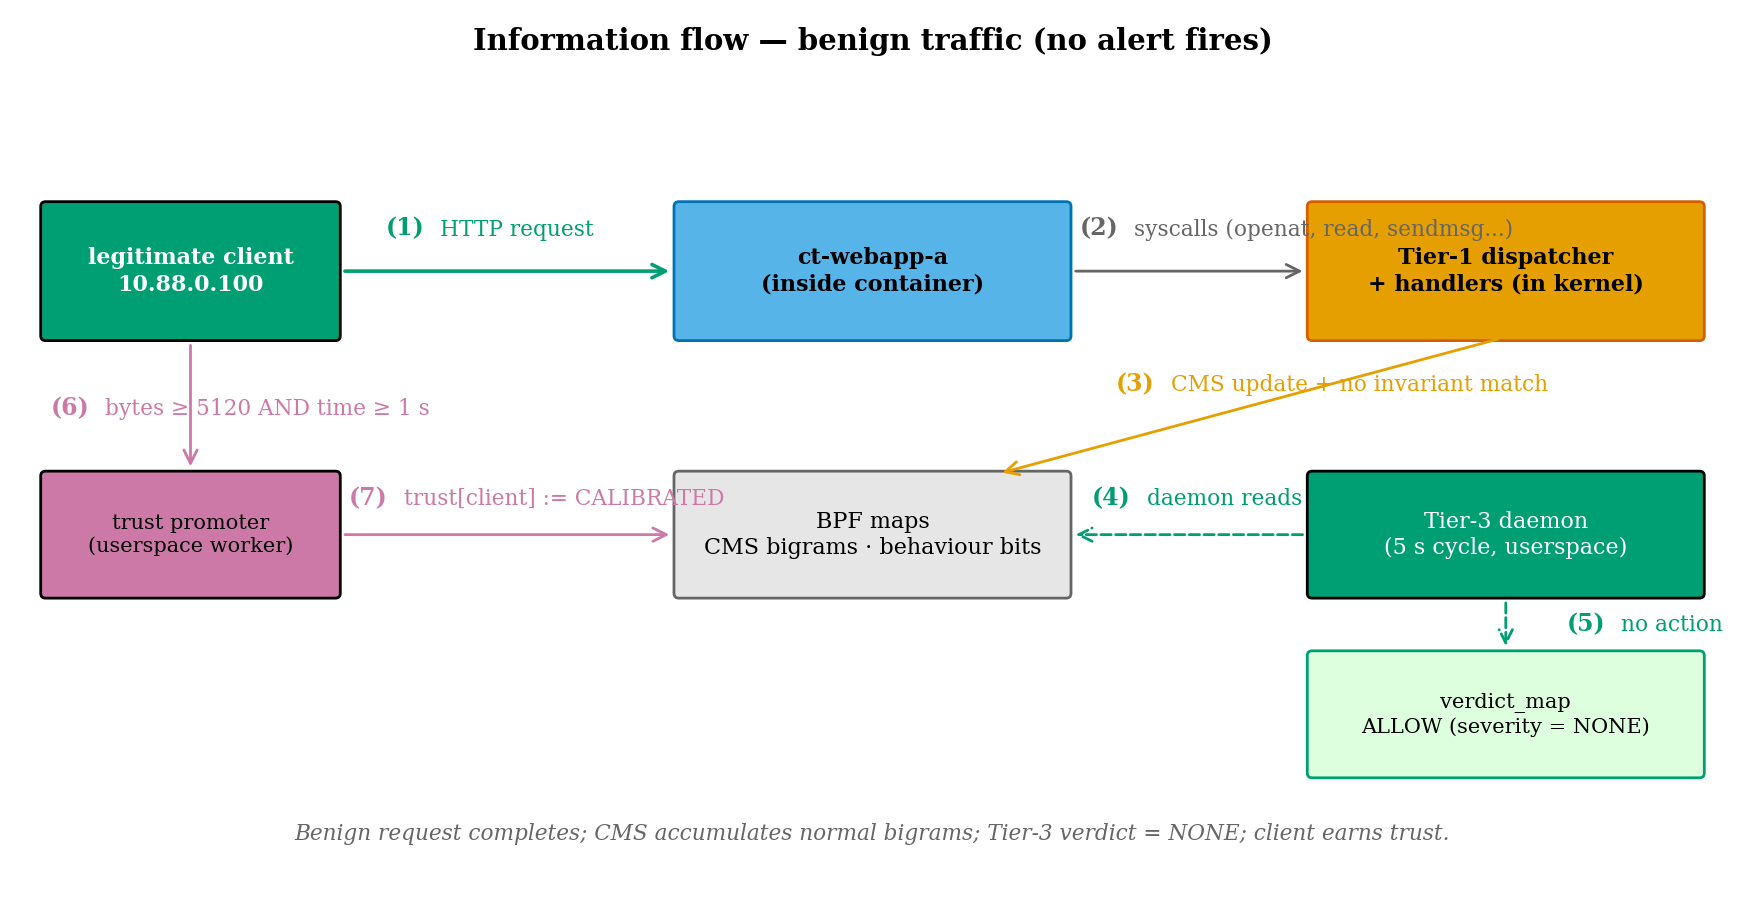
\includegraphics[width=\linewidth]{figures/fig_dataflow_normal.png}
  \caption[Normal-traffic data flow]{Information flow on benign traffic. The
  client issues an HTTP request (1); syscalls reach the Tier-1 dispatcher
  (2); the CMS is updated but no invariant matches (3); Tier-3 reads the
  accumulated state on its next cycle (4) and writes an \textsc{Allow}
  verdict (5); meanwhile the trust promoter observes flow stability (6--7)
  and upgrades the client to \textsc{Calibrated}. No kill, no drop.}
  \label{fig:dataflow-normal}
\end{figure}

\begin{figure}[t]
  \centering
  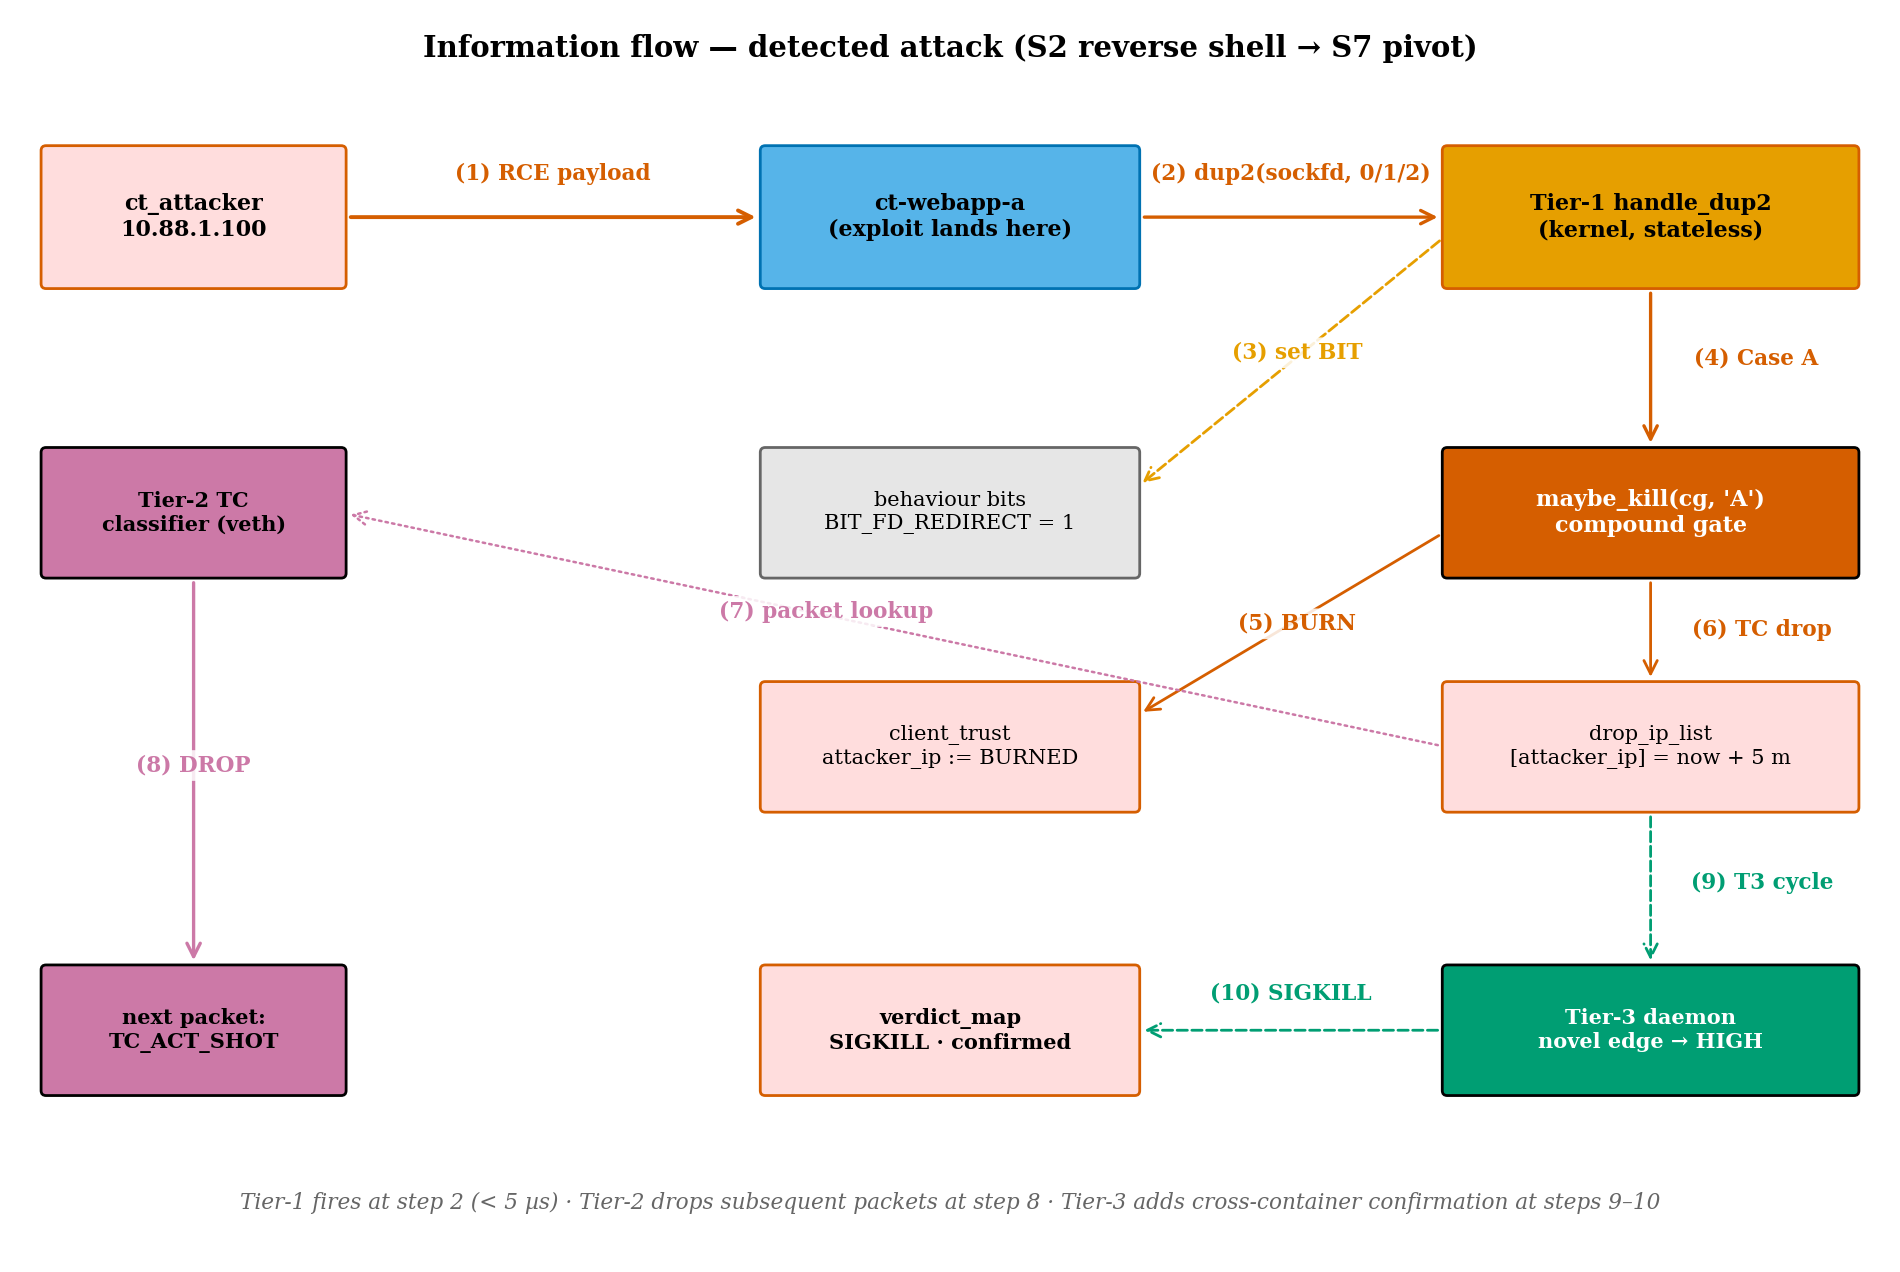
\includegraphics[width=\linewidth]{figures/fig_dataflow_attack.png}
  \caption[Attack data flow]{Information flow on a detected attack. An RCE
  payload lands in a webapp (1--2); \texttt{handle\_dup2} fires on the
  socket-to-stdio \texttt{dup2} (3--4); the compound gate writes the
  attacker IP into \texttt{drop\_ip\_list} and burns the trust entry (5--6);
  the TC classifier drops all subsequent attacker packets at the veth (7--8);
  Tier-3's next cycle produces an independent cross-container confirmation
  (9--10). Tier-1 acts in the sub-microsecond regime; Tier-2 severs the
  session at the network layer within a packet; Tier-3 adds graph-level
  evidence on the 5-second cadence.}
  \label{fig:dataflow-attack}
\end{figure}

%─────────────────────────────────────────────────────────────────────────────
\section{Threat model}
\label{sec:threat}
%─────────────────────────────────────────────────────────────────────────────

Figure~\ref{fig:threat-model} summarises the scope. The primary asset is
the confidentiality, integrity, and availability of the monitored
containers' workloads and of the database tier's data at rest. Secondary
assets are the host's other tenants (no cross-container leakage) and the
host itself (no escape to the root namespace).

\begin{figure}[t]
  \centering
  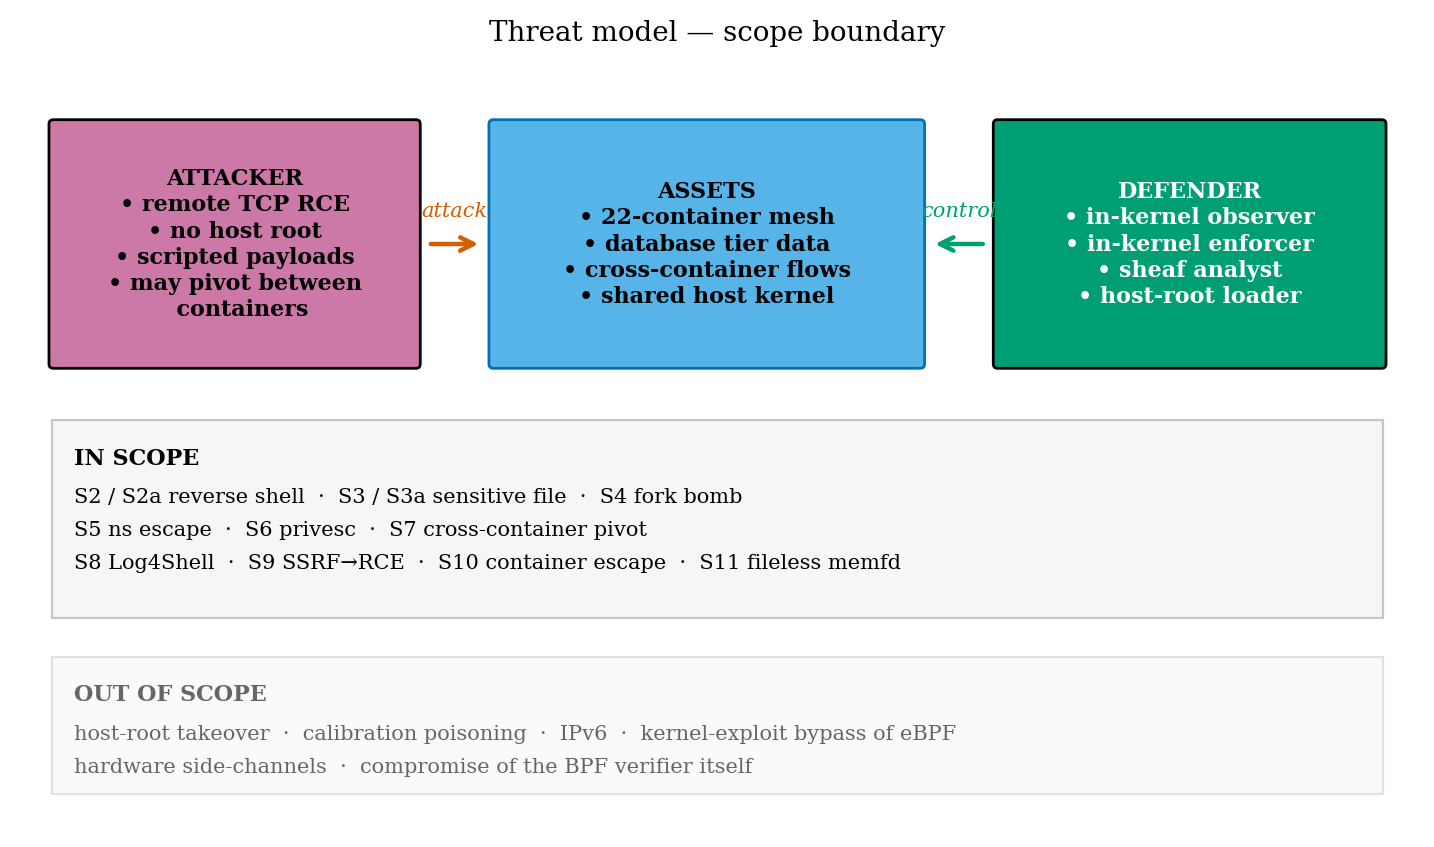
\includegraphics[width=0.88\linewidth]{figures/fig_threat_model.png}
  \caption[Threat-model scope]{In-scope attacks (S2 through S11) and
  explicit out-of-scope assumptions. The defender operates inside the
  kernel and assumes host root is not compromised.}
  \label{fig:threat-model}
\end{figure}

\paragraph{Adversary capability.} The adversary has code execution inside a
monitored container, at the privilege level of the container's main
process. The adversary can originate this code execution either from
outside through a network vulnerability (RCE, SSRF, Log4Shell-class)
or by pivoting from a peer container that was compromised first. The
adversary does not hold host root.

\paragraph{Out of scope.} We exclude: attackers with host root (who can
unload BPF programs directly); attackers with a kernel exploit that writes
kernel memory outside the BPF verifier's model; attackers who subvert the
BPF verifier itself; denial-of-service attacks that overwhelm the ring
buffers before any alert can escape. These are legitimate attack classes
but lie outside what an in-kernel defender can defeat.

\paragraph{Defender capability.} We assume a host-root loader that attaches
the eBPF programs at boot, a Python daemon with access to BPF maps (running
as the same UID as the loader), and network administrator capability
(\texttt{CAP\_NET\_ADMIN}) to attach TC filters to container veths.

%─────────────────────────────────────────────────────────────────────────────
\section{Three-tier architecture}
\label{sec:tiers}
%─────────────────────────────────────────────────────────────────────────────

We enumerate the three tiers in data-flow order.

\textbf{Tier~1 (kernel, stateless).} A raw tracepoint attached to
\texttt{sys\_enter} sees every syscall issued by every process on the host.
A dispatcher filters out host processes via mount-namespace comparison,
updates a per-cgroup Count-Min Sketch of the syscall bigram, and tail-calls
to one of six specialist handlers based on the syscall opcode. Each
handler tests a physical invariant (dup2 socket-to-stdio, shell-exec with
socket-fd, setuid(0) from non-root, unshare with CLONE\_NEWNS, path-class
match on openat, fork acceleration) and either returns without action,
updates a behaviour bit in a shared map, or enters the compound-gate
decision of Section~\ref{sec:compound}.

\textbf{Tier~2 (kernel, attribution).} Two kprobes
(\texttt{tcp\_v4\_connect} and \texttt{inet\_csk\_accept}) and two pairs of
byte-accounting kprobes (\texttt{tcp\_sendmsg}/\texttt{tcp\_recvmsg})
attribute every network byte to a remote peer IP. A per-TID LRU map of
16,384 slots keeps the attribution fresh across fork-exec worker patterns.
A per-socket context map of 8,192 slots accumulates byte counts for the
L4-stability-based trust promotion described in Section~\ref{sec:trust-model}.
When the compound gate decides to sever an attacker's session, Tier~2
writes the attacker IP to \texttt{drop\_ip\_list} with a 5-minute TTL, and
the direct-action TC classifier on each container's veth silently returns
\texttt{TC\_ACT\_SHOT} for any packet matching the burned IP.

\textbf{Tier~3 (user-space, analytics).} A Python daemon reads the
Count-Min Sketches and behaviour bits from the kernel every five seconds,
extracts the 74-dimensional signal per container, computes the Mahalanobis
edge energies and the global Rayleigh quotient through the mathematics of
Chapter~\ref{Chapter3}, and writes verdicts to a JSONL log. The daemon may
also write into the enforcement maps (\texttt{deny\_connect\_map},
\texttt{deny\_openat\_map}, \texttt{fw\_allow\_map}, etc.) to graduate
enforcement under confirmed anomalies. Tier~3 is optional: the kernel
continues to enforce strict invariants regardless of daemon state.

\paragraph{The independence invariant.} The three tiers communicate only
through BPF maps. Tier~1 never blocks on Tier~3. Tier~3 never blocks
Tier~1. If the Python daemon crashes, segfaults, or runs out of memory,
Tier~1 and Tier~2 remain attached and enforcing; the only degradation is
the loss of the sheaf-coupling detection surface. This decoupling is the
structural answer to research gap~G3 (detection-vs-enforcement split) from
Chapter~\ref{Chapter2}.

%─────────────────────────────────────────────────────────────────────────────
\section{Tier~1: the dispatcher and six handlers}
\label{sec:tier1}
%─────────────────────────────────────────────────────────────────────────────

The Tier~1 dispatcher runs six steps on every syscall:

\begin{enumerate}
  \item Read the syscall number from \texttt{ctx->args[1]}.
  \item Compute the current task's mount namespace inode and compare against
    the single-slot \texttt{host\_ns} array. Host-side processes return
    immediately.
  \item Check the cgroup's verdict map for a Tier~3 KILL decree and
    SIGKILL if present.
  \item Resolve pending cgroup inheritance (for post-unshare children).
  \item Update the Count-Min bigram sketch (unless this syscall is on the
    noise list of \texttt{getpid}, \texttt{gettid}, \texttt{getuid},
    \texttt{getppid}, \texttt{time}, \texttt{clock\_gettime}).
  \item Tail-call through \texttt{prog\_array[syscall\_nr]} to the
    specialist handler.
\end{enumerate}

The tail-call is an unconditional branch; cold paths where no specialist
handler is registered for the opcode still fall through to the map lookup
and simply return 0 from the program-array call. This keeps the hot-path
overhead to a single comparison plus an indirect branch, measured at
approximately 65\,ns on our evaluation kernel.

The six handlers cover the strict-invariant attack classes we target:

\begin{description}
  \item[\texttt{handle\_dup2}] inspects \texttt{dup2(oldfd, newfd)}. If
    \texttt{newfd} is 0, 1, or 2 and the file pointed to by \texttt{oldfd}
    is a socket (\texttt{i\_mode \& 0xF000 == S\_IFSOCK}), the handler
    sets \texttt{BIT\_FD\_REDIRECT}, emits an alert, and calls
    \texttt{maybe\_kill(cg, 'A')}. No legitimate workload redirects stdio
    onto a socket.

  \item[\texttt{handle\_fork}] counts \texttt{clone(2)} and
    \texttt{clone3(2)} per-cgroup per-second. The handler computes the
    second discrete derivative $d^2 = \text{rate}_t - 2\,\text{rate}_{t-1}
    + \text{rate}_{t-2}$ and fires when $d^2 > 0$ is sustained with
    monotonic growth, or when the raw rate exceeds 500/s. The second
    derivative catches the acceleration phase before the absolute rate
    reaches fork-bomb territory. This is a self-inflicted kill; Case~D in
    the compound gate.

  \item[\texttt{handle\_execve}] extracts the basename of the exec'd
    filename (in-kernel byte-by-byte string comparison because eBPF
    forbids \texttt{strcmp}) and matches against \{\texttt{sh, bash,
    dash, nc, ncat, zsh}\}. If the binary is a shell, the handler
    inspects fds 0, 1, 2: if any is a socket, this is a reverse shell
    staged through shell redirection (\texttt{bash -i >\&
    /dev/tcp/host/port}), a strict invariant. Otherwise, plain shell
    exec is Case~X, trust-gated.

  \item[\texttt{handle\_file}] (\texttt{openat}) and \texttt{handle\_file\_open}
    (\texttt{open}) classify the requested path against a pruned trie:
    \texttt{/etc/sha} prefix $\to$ sensitive-credentials read;
    \texttt{/proc/1/} prefix $\to$ namespace probe; \texttt{/var/run/sec}
    prefix $\to$ Kubernetes secrets. The handler sets the matching bit
    but does not kill (file-reads alone are ambiguous; we defer to the
    compound gate with Tier~3 confirmation).

  \item[\texttt{handle\_privesc}] dispatches on syscall number:
    \texttt{setuid(105)} $\to$ check that target uid is 0 and current uid
    is non-zero $\to$ Case~A. \texttt{unshare(272)} $\to$ check for
    CLONE\_NEWNS or CLONE\_NEWUSER flags $\to$ Case~A. \texttt{setns(308)}
    and \texttt{ptrace(101)} $\to$ unconditional Case~A inside a
    container.

  \item[\texttt{trace\_connect\_return}] (not strictly a tail-called handler
    but part of the Tier~1 enforcement surface). On successful
    \texttt{tcp\_v4\_connect}, the handler looks up the destination
    container via \texttt{ip\_to\_cgroup}. If the source cgroup already
    has \texttt{BIT\_SHELL\_SPAWN} or \texttt{BIT\_FD\_REDIRECT} set
    within the last 5~s, this is a compound confirmed two-hop attack
    and the handler calls \texttt{maybe\_kill(src\_cg, 'A')}.
\end{description}

Each handler's hot path completes in the 280--640\,ns band on the
evaluation host (Intel Core i7-10710U, kernel~6.17, BCC-compiled BPF).
Figure~\ref{fig:tier1-detail} shows the full dispatcher/handler/gate
topology; every handler is a tail-call from the dispatcher and every
enforcement request funnels through \texttt{maybe\_kill}.

\begin{figure}[t]
  \centering
  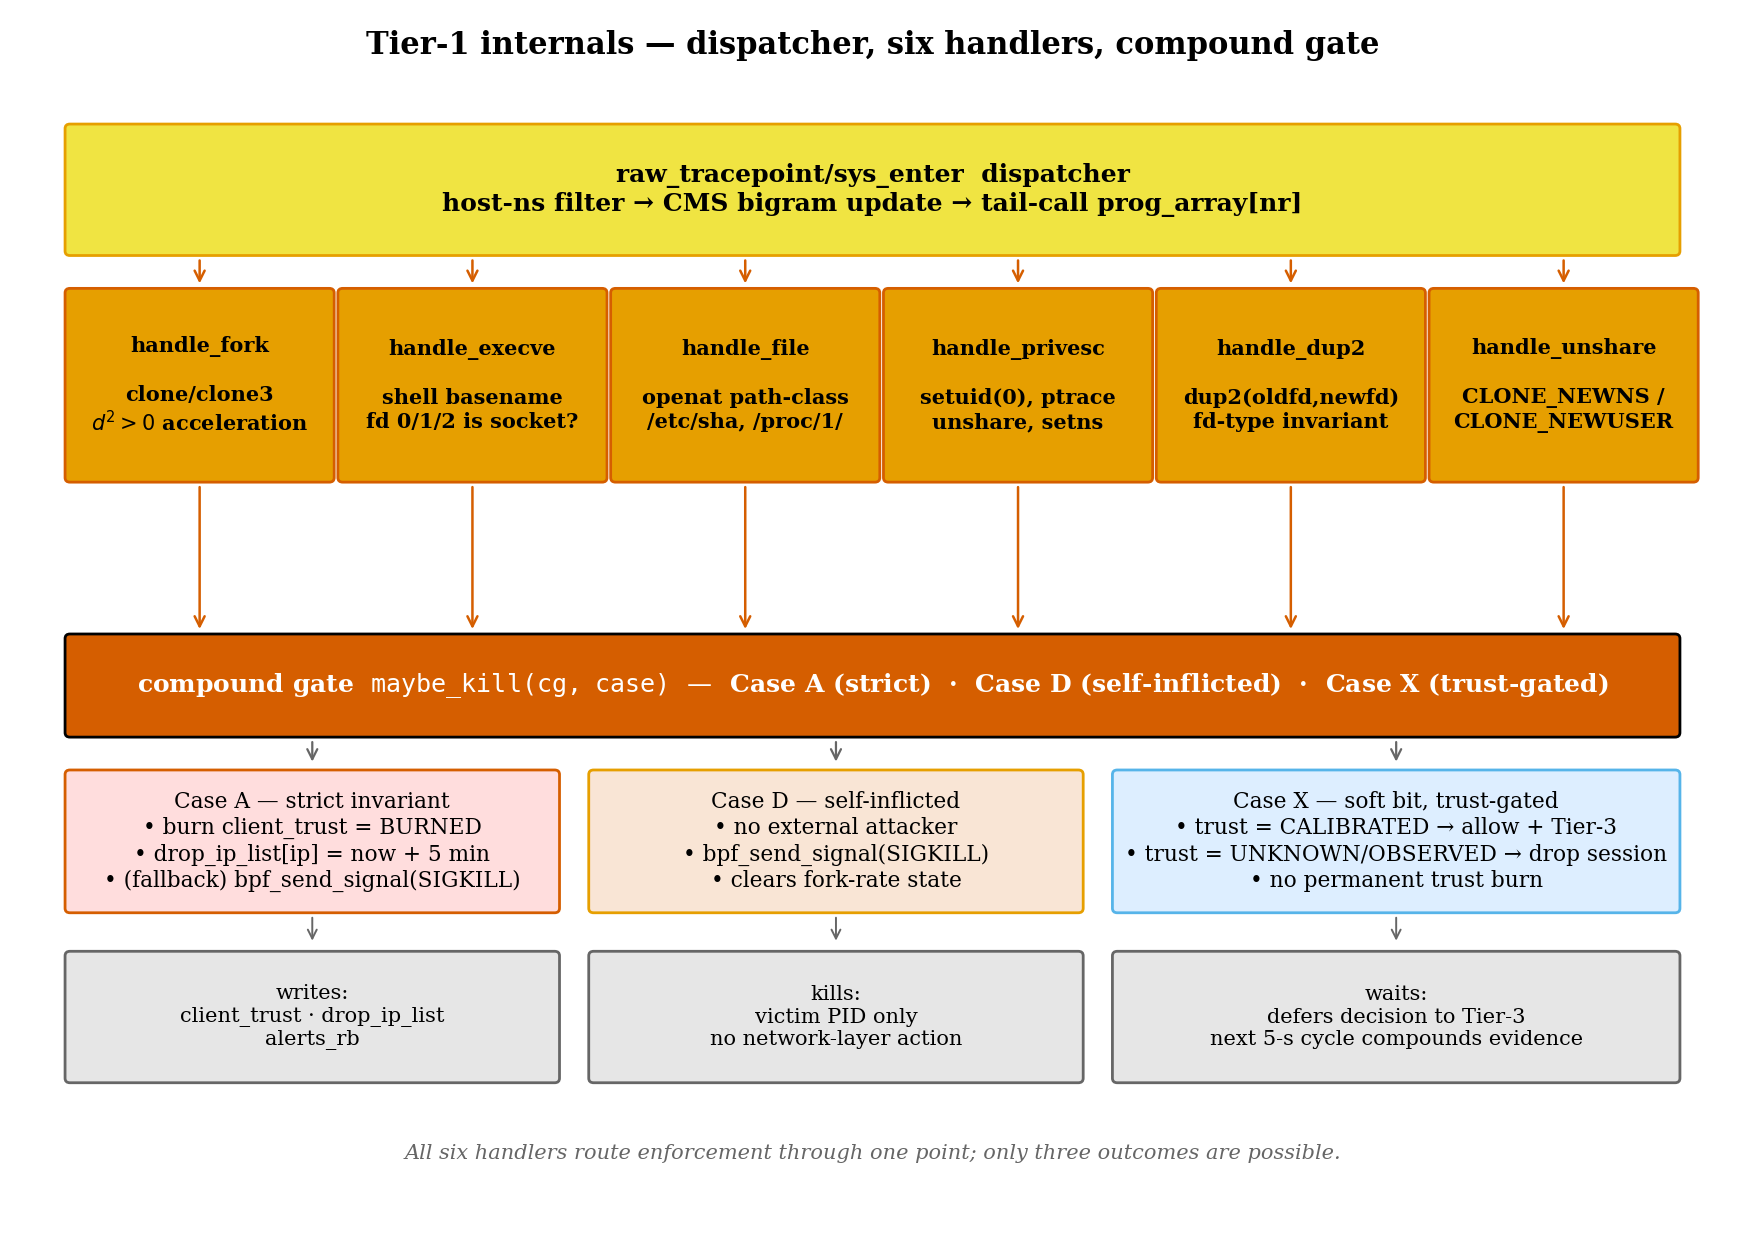
\includegraphics[width=\linewidth]{figures/fig_arch_tier1_detail.png}
  \caption[Tier-1 internals]{Tier-1 dispatcher, the six specialist
  handlers, and the compound gate. The dispatcher performs the host-ns
  filter and CMS bigram update, then tail-calls the opcode-specific
  handler. Every handler terminates at \texttt{maybe\_kill(cg, case)};
  the gate routes to exactly one of three outcomes (Case A / D / X).}
  \label{fig:tier1-detail}
\end{figure}

%─────────────────────────────────────────────────────────────────────────────
\section{The compound enforcement gate}
\label{sec:compound}
%─────────────────────────────────────────────────────────────────────────────

The compound gate \texttt{maybe\_kill(cg, case)} is the single kill
decision point in the kernel. All six handlers funnel enforcement requests
through it. The gate takes a cgroup identifier and a \emph{case tag} that
classifies the triggering event:

\begin{description}
  \item[Case A (Strict invariant).] Physical contract violation: dup2
    socket-to-stdio, shell exec with socket stdio, setuid(0), unshare
    with namespace flags, two-hop compound. The gate burns the
    attacker's client IP (if attributable) into \texttt{client\_trust}
    and writes the IP into \texttt{drop\_ip\_list} with a 5-minute TTL.
    If the client IP is not attributable (some strict invariants have no
    external attacker), the gate falls back to \texttt{bpf\_send\_signal(SIGKILL)}.

  \item[Case D (Self-inflicted).] Fork bomb, runaway workload. No external
    attacker to drop at the veth. The gate sends \texttt{SIGKILL} to
    stop the workload.

  \item[Case X (Soft-bit, trust-gated).] Plain shell exec, single
    sensitive-file read, single lateral connect to an uncalibrated port
    without an accompanying invariant. The gate reads the client IP's
    trust level. If CALIBRATED, the gate returns without action and
    relies on Tier~3 to compound-confirm; if UNKNOWN, OBSERVED, or
    BURNED, the gate treats the event as Case~C: write the IP to
    \texttt{drop\_ip\_list}, but do not burn trust permanently.
\end{description}

This three-case taxonomy reflects a design observation: different
categories of evidence merit different enforcement targets. Physical
invariants warrant permanent trust burn plus session drop. Self-inflicted
events warrant stopping the workload. Soft anomalies from trusted clients
warrant waiting for compound confirmation rather than silent collateral
damage. Legacy designs that compressed all three into a single
\texttt{SIGKILL(process)} pathway suffered G4 (coarse enforcement target).

\begin{figure}[t]
  \centering
  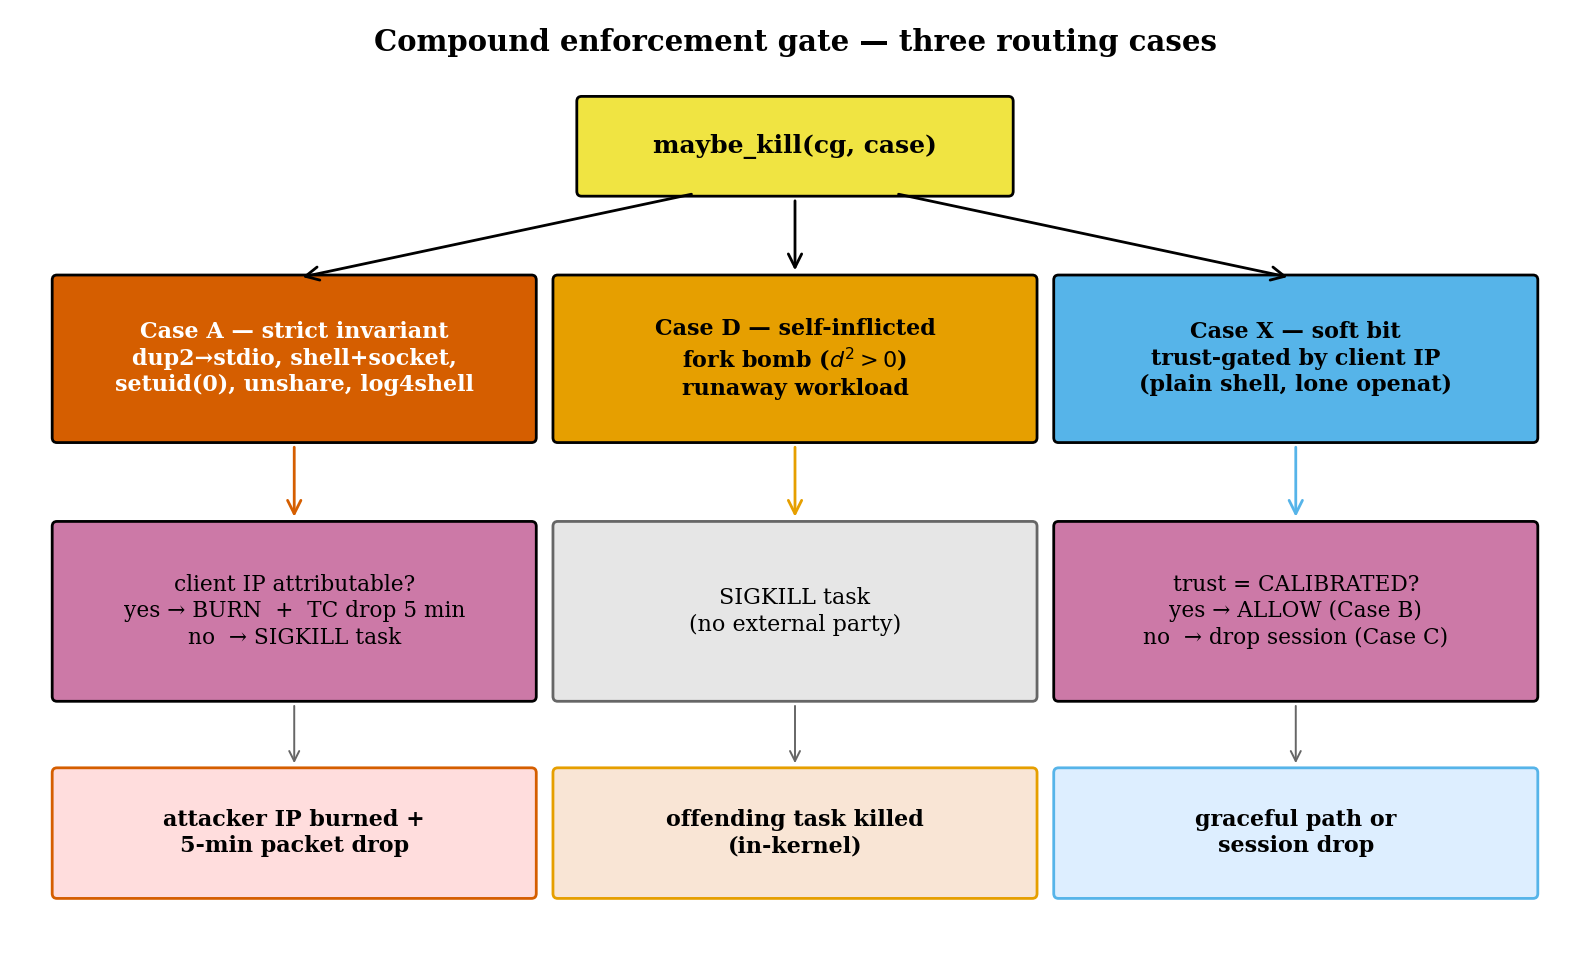
\includegraphics[width=0.88\linewidth]{figures/fig_compound_gate.png}
  \caption[Compound enforcement gate]{Three routing cases of
  \texttt{maybe\_kill(cg, case)}. Case~A burns the attacker's IP and
  drops all its packets at the veth (SIGKILL is a fallback when no IP is
  attributable). Case~D kills the offending task because no external
  attacker exists. Case~X reads trust state and takes a grace path for
  calibrated clients or drops the session otherwise.}
  \label{fig:gate}
\end{figure}

Table~\ref{tab:invariants} closes the loop on Theorem~\ref{thm:invariant}
by mapping each attack scenario to the invariant that catches it.

\begin{table}[t]
\centering
\caption[Per-scenario invariants]{Attack scenarios and the Tier-1 invariant
that catches each. Every row is the necessary-condition claim of
Theorem~\ref{thm:invariant} realised in a kernel hook.}
\label{tab:invariants}
\small
\begin{tabular}{llll}
\toprule
ID & Scenario & Necessary syscall pattern & Kernel handler \\
\midrule
S2   & Reverse shell         & \texttt{dup2(sockfd, 0|1|2)}    & \texttt{handle\_dup2} \\
S2a  & Revshell + noise pad  & \texttt{dup2(sockfd, 0|1|2)}    & \texttt{handle\_dup2} \\
S3   & \texttt{/etc/shadow} read
                              & \texttt{openat("/etc/sha*")}    & \texttt{handle\_file} \\
S3a  & Sensitive + noise pad & \texttt{openat("/etc/sha*")}    & \texttt{handle\_file} \\
S4   & Fork bomb             & $d^2(\text{rate})/dt^2 > 0$     & \texttt{handle\_fork} \\
S5   & Namespace escape      & \texttt{nsenter}\,$\to$\,\texttt{setns(fd,\,\_NEWNS)}
                                                               & \texttt{handle\_privesc} \\
S6   & Privilege escalation  & \texttt{unshare(\_NEWUSER|\_NEWNS)}\,+\,\texttt{setuid(0)}
                                                               & \texttt{handle\_privesc} \\
S7   & Cross-container pivot & \textsc{Tier-1} two-hop + \textsc{Tier-3} sheaf
                                                               & \texttt{trace\_connect\_return} \\
S8   & Log4Shell chain       & \texttt{execve(shell)} + socket
                                                               & \texttt{handle\_execve} \\
S9   & SSRF $\rightarrow$ RCE
                              & \textsc{Tier-3} sheaf edge spike
                                                               & \texttt{sheaf\_detector} \\
S10  & Container escape      & rare-syscall chain: \texttt{unshare}, \texttt{mount},
                                \texttt{core\_pattern} write, \texttt{memfd+exec}, \texttt{bpf()}
                                                               & \texttt{handle\_privesc} + Top-24 \\
S11  & \texttt{memfd\_create} OOD
                              & \texttt{execveat(/proc/self/fd/N)}
                                                               & \texttt{handle\_execve} \\
\bottomrule
\end{tabular}
\end{table}

%─────────────────────────────────────────────────────────────────────────────
\section{Tier~2: attribution and session severance}
\label{sec:tier2}
%─────────────────────────────────────────────────────────────────────────────

Tier~2's job is to make the compound gate's decision targetable. Two
structures support this.

\paragraph{Attribution.} The per-TID LRU map \texttt{tid\_client\_ip} (16,384
slots) records the client IP from which each thread received its
most-recent work. The map is populated on \texttt{inet\_csk\_accept}:
the accepting thread's pid/tgid is the key, the peer IP extracted from
\texttt{sock->\_\_sk\_common.skc\_daddr} is the value. A fork hook
(\texttt{sched\_process\_fork} tracepoint) propagates the attribution from
parent to child so that forked workers inherit the IP of the request that
spawned them. A per-cgroup fallback map \texttt{cgroup\_current\_client}
records the most recent accepted IP per cgroup; it serves as a
best-effort fallback when per-TID attribution misses (for instance in
accept-thread-plus-thread-pool servers).

\paragraph{Trust promotion.} The trust promoter (a userspace worker, not
in the kernel hot path) reads the per-socket byte-accumulation map
\texttt{connection\_context} every few seconds. A client IP is promoted
from OBSERVED to CALIBRATED when any single flow from that IP accumulates
$\geq 5120$~bytes and runs for $\geq 1$~second (the L4-stability rule).
This simple rule distinguishes a client that completes a real HTTP
transaction from one that merely opens a TCP connection and disconnects.
A client IP is permanently demoted to BURNED when any Case~A strict
invariant fires on a syscall attributed to that IP.

\paragraph{Session severance at the veth.} When the compound gate decides
to drop an attacker, it writes the attacker IP to \texttt{drop\_ip\_list}
with expiry \texttt{bpf\_ktime\_get\_ns()\,+\,5 min}. A TC classifier
program, attached via \texttt{tc filter add dev <veth> ingress/egress bpf
direct-action} to every monitored container's host-side veth, consults
\texttt{drop\_ip\_list} on every packet: if the source (on ingress) or
destination (on egress) IP matches an unexpired entry, the classifier
returns \texttt{TC\_ACT\_SHOT} and the packet is silently dropped. The
TC program's hot path is approximately 100~ns; the full severance latency
from invariant fire to first-packet drop is below 1\,$\mu$s.

\paragraph{Why not \texttt{sockops} TCP RST?} An alternative we
considered was injecting a TCP~RST through the \texttt{sockops} hook to
tear down the attacker's session explicitly. Two considerations rule
this out. First, the attacker's TCP stack may ignore or slow-retry a
single RST, whereas unconditional packet drop is terminal. Second,
\texttt{sockops} requires kernel support for the specific RST-injection
path (not universally available across the kernel 5.x--6.x range), while
TC direct-action has been stable since kernel~4.18. The drop-based
mechanism is simpler, more universal, and easier to reason about.

%─────────────────────────────────────────────────────────────────────────────
\section{Tier~3: the sheaf daemon}
\label{sec:tier3}
%─────────────────────────────────────────────────────────────────────────────

Every five seconds, the Tier~3 daemon runs one detection cycle:

\begin{enumerate}
  \item Read the Count-Min Sketch for every monitored cgroup from the BPF
    map \texttt{bigram\_sketch\_map}. Reconstruct the 625-dimensional
    bigram vector per container.
  \item Read the behaviour-bit snapshot from
    \texttt{container\_behavior}.
  \item Drain the connection event telemetry from the 256-KiB ring
    buffer \texttt{telemetry\_rb}.
  \item Extract the 74-dimensional signal per container (entropy + PCA +
    top-20 marginals + rate) and whiten per container using the stored
    means and standard deviations.
  \item For every calibrated edge $e = (u, v, \ell) \in E$, compute
    $\mathbf{r}_e = F_u^{(e)}\,\tilde{\mathbf{x}}_u - F_v^{(e)}\,\tilde{\mathbf{x}}_v$,
    the Mahalanobis energy $E_e = \mathbf{r}_e^\top \Sigma_e^{-1} \mathbf{r}_e$,
    and flag if $E_e > \tau_e$.
  \item Compute the global Rayleigh quotient $R$ from the full stacked
    signal and compare against the guarded-EMA threshold $\tau^{(t)}$.
  \item Run the compound-confirmation logic: if any edge was flagged AND
    the global gate fired AND a behaviour bit is live in any of the
    edge's incident containers, escalate enforcement via
    \texttt{enforce\_level\_map} (graduated L0--L6 levels described in
    Chapter~\ref{Chapter5}).
  \item Write a verdict record to \texttt{results/causaltrace/verdicts.jsonl}.
  \item Update the guarded EMA only if all six previous cycles were
    pristine.
\end{enumerate}

The detection cycle completes in approximately 50--200\,ms on the
evaluation host, bounded by CCA projection and covariance inverse
applications. The 5-second cadence gives ample slack; the daemon spends
roughly 2\,\% of wall-clock time running. Figure~\ref{fig:sliding-window}
visualises the cycle structure and the eight internal steps of each
detection pass.

\begin{figure}[t]
  \centering
  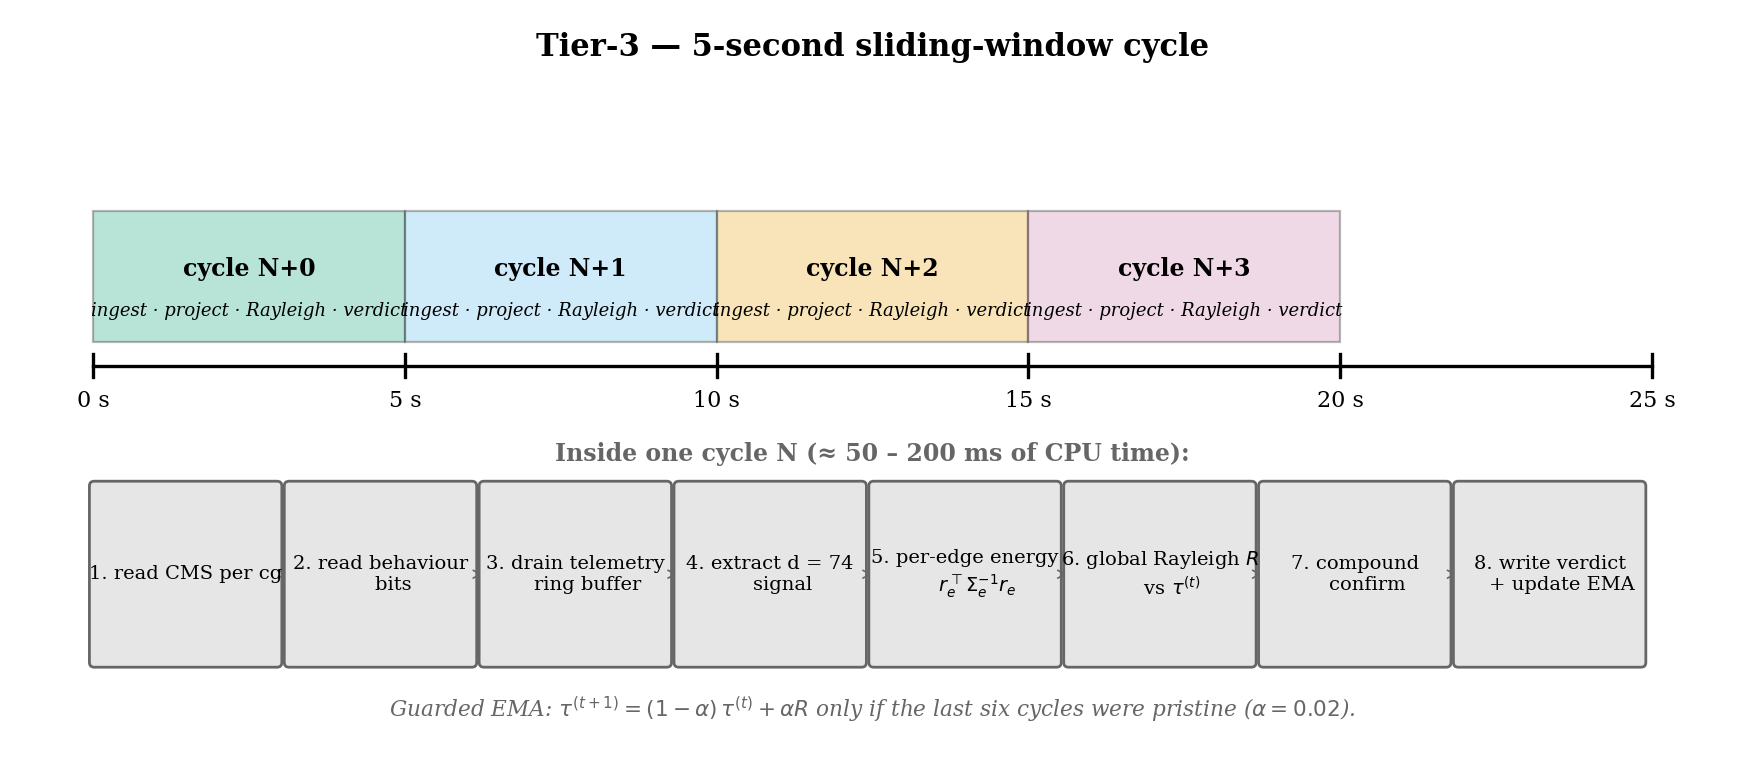
\includegraphics[width=\linewidth]{figures/fig_sliding_window.png}
  \caption[Tier-3 detection cycle]{Tier-3 sliding-window structure. The top
  timeline shows consecutive five-second cycles. The bottom row expands
  one cycle into its eight internal steps: map read, behaviour-bit
  snapshot, telemetry drain, signal extraction, per-edge Mahalanobis
  energy, global Rayleigh comparison, compound confirmation, and verdict
  write. The guarded EMA advances only after six pristine cycles.}
  \label{fig:sliding-window}
\end{figure}

%─────────────────────────────────────────────────────────────────────────────
\section{Trust model}
\label{sec:trust-model}
%─────────────────────────────────────────────────────────────────────────────

Client IPs move through the four-state automaton shown in
Figure~\ref{fig:trust-fsm}. \textsc{Unknown} is the default. \textsc{Observed}
means at least one TCP accept from that IP. \textsc{Calibrated} requires an
L4-stability pass ($\geq 5120$~B and $\geq 1$~s on a single flow), which is
what Theorem~\ref{thm:trust} rests on. \textsc{Burned} is set by any Case~A
strict invariant and cannot be rehabilitated during the current run.

\begin{figure}[t]
  \centering
  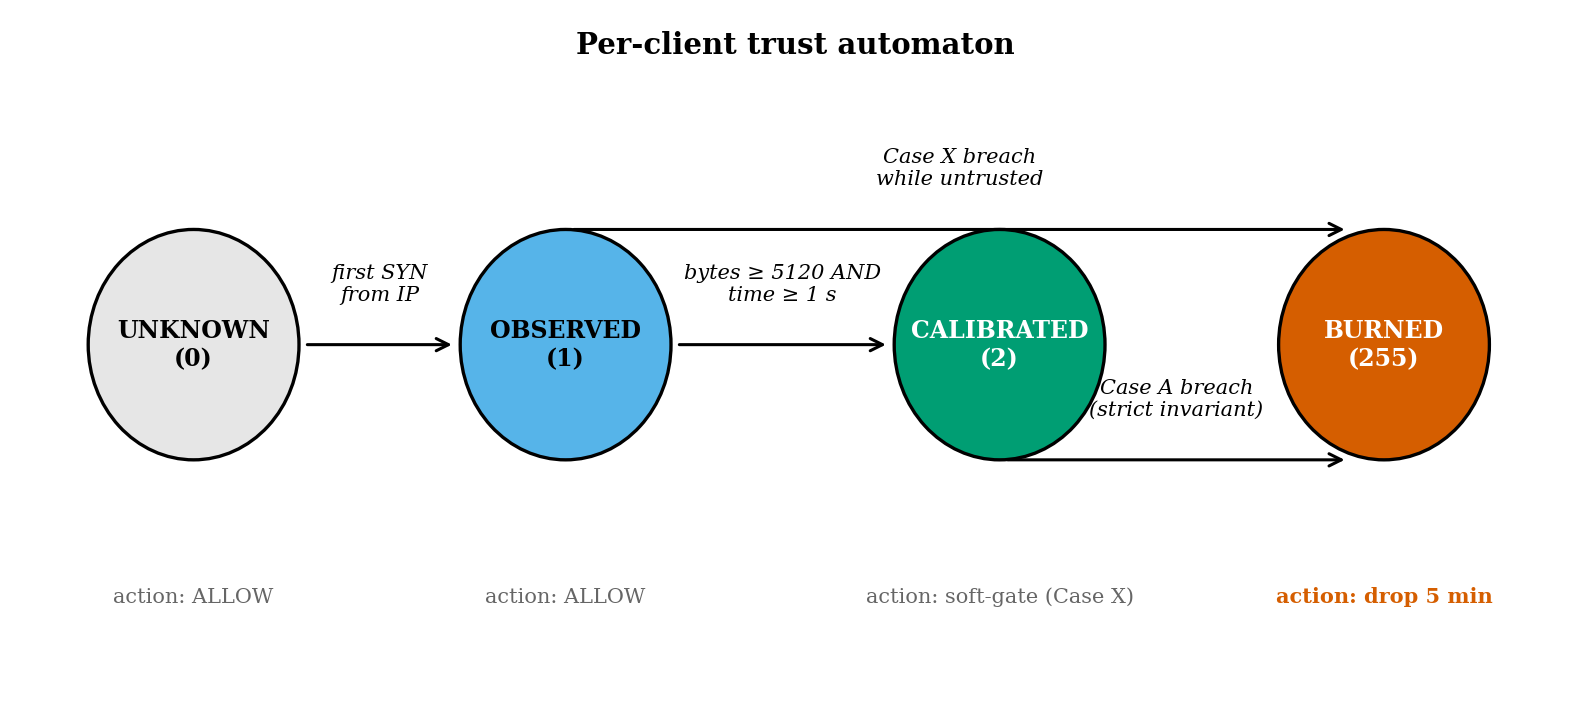
\includegraphics[width=0.92\linewidth]{figures/fig_trust_state_machine.png}
  \caption[Per-client trust FSM]{Four-state trust automaton per client IP.
  Transitions are monotonic except $\text{any} \to \textsc{Burned}$, which
  overwrites a prior \textsc{Calibrated} promotion.}
  \label{fig:trust-fsm}
\end{figure}

The compound gate reads \texttt{client\_trust[client\_ip]} on every Case~X
decision and routes \textsc{Calibrated} clients to the alert-only path,
everyone else to the drop-session path.

%─────────────────────────────────────────────────────────────────────────────
\section{Testbed topology}
\label{sec:testbed}
%─────────────────────────────────────────────────────────────────────────────

Figure~\ref{fig:testbed} shows the evaluation topology. Twenty-two
containers run across two bridge networks: \texttt{ct\_prod\_net}
(\texttt{10.88.0.0/24}) carries eighteen workload services plus the
legitimate load generator \texttt{ct\_legit\_client} on \texttt{.100};
\texttt{ct\_attack\_net} (\texttt{10.88.1.0/24}) isolates
\texttt{ct\_attacker} on \texttt{.100} from the prod net's default routes.

\begin{figure}[t]
  \centering
  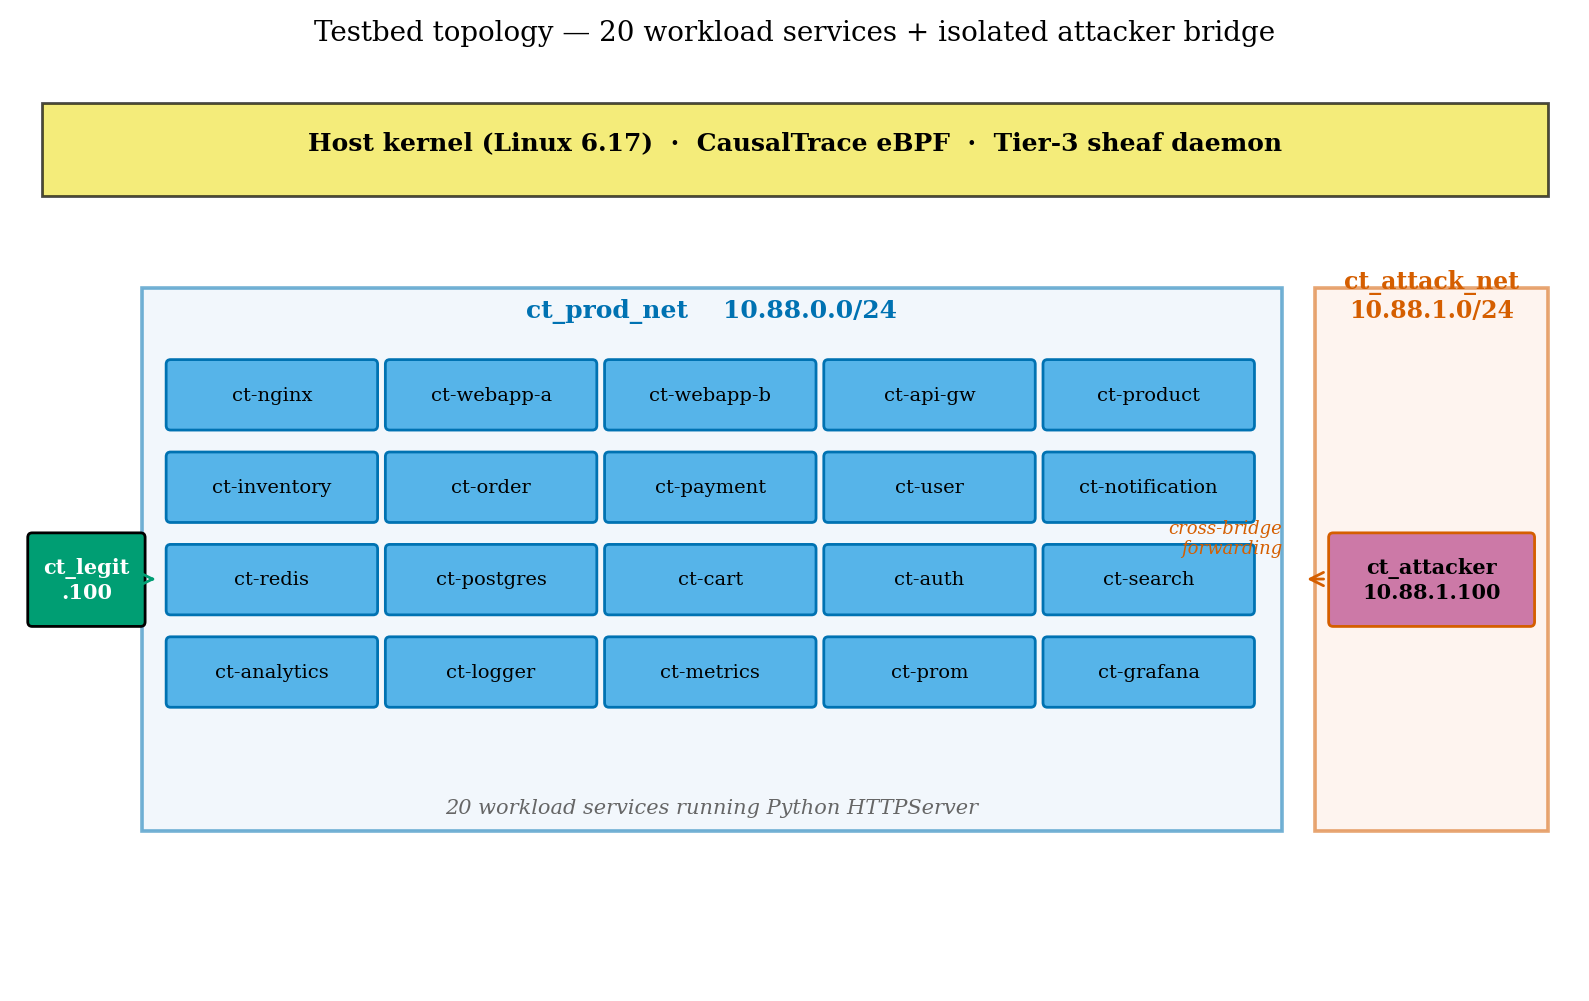
\includegraphics[width=\linewidth]{figures/fig_testbed_topology.png}
  \caption[Testbed topology]{22-container evaluation testbed. Workload
  services run Python \texttt{HTTPServer} on the \texttt{ct\_prod\_net}
  bridge. The attacker is on a separate bridge to force cross-bridge
  routing (source IP survives masquerade is disabled) and to keep the
  attacker IP out of the calibrated range.}
  \label{fig:testbed}
\end{figure}

Masquerade is disabled on both bridges
(\texttt{com.docker.network.bridge.enable\_ip\_masquerade: false}) so
source IPs survive cross-bridge routing. IPv6 is disabled everywhere
because Probe~B only hooks \texttt{tcp\_v4\_connect}. Inter-bridge
forwarding is enabled by \texttt{scripts/setup\_routes.sh}, which also
cleans up Docker's nftables raw-table drops.

During calibration, \texttt{ct\_legit\_client} earns
\texttt{trust = CALIBRATED} by running a sustained \texttt{wrk} workload
against every service, generating L4-stable flows. The attacker container
starts fresh with \texttt{trust = UNKNOWN}, so every attack injection
forces the compound gate down the untrusted-anomaly path.

%─────────────────────────────────────────────────────────────────────────────
\section{Calibration workflow}
\label{sec:calibration}
%─────────────────────────────────────────────────────────────────────────────

Calibration is a one-shot offline process per testbed deployment, driven
by \texttt{scripts/calibration\_driver.py} in four stages.

\begin{enumerate}
  \item Bring the testbed to healthy state and attach the loader in
    calibration mode; the loader compiles the BCC program, attaches the
    dispatcher, the six handlers, and the Tier-2 probes, and starts the
    telemetry ring-buffer reader.
  \item Drive legitimate traffic: concurrent \texttt{wrk} workers hammer
    every service at the host edge while a second generator issues
    inter-service \texttt{docker exec} calls that exercise every edge of
    the communication graph.
  \item Call \texttt{SheafCalibrator.calibrate()} with the accumulated
    bigram traces and connection events; the calibrator fits the PCA
    projection ($625 \to 50$), the per-container whiteners, CCA
    restriction maps at three lags per edge, the regularised edge
    covariances, the per-edge Mahalanobis thresholds, and the global
    Rayleigh threshold.
  \item Serialise every artefact to \texttt{calibration/}
    (\texttt{pca.pkl}, \texttt{whiteners.pkl},
    \texttt{restriction\_maps.npz}, \texttt{edge\_thresholds.json},
    \texttt{global\_threshold.json}, \texttt{calibrated\_edges.json}).
\end{enumerate}

A fresh calibration on our testbed produced 42 calibrated edges, 102
edge-lag Mahalanobis thresholds (median $\hat\tau = 73.5$, range
50.7--103.9), and a global Rayleigh threshold
$\tau_{\text{global}} = 0.78$. Chapter~\ref{Chapter6} reports these values
alongside their runtime-detection consequences.
